\documentclass[compsoc]{IEEEtran}
\usepackage{graphicx}
\usepackage{amsmath}
\usepackage{authblk}
\usepackage[english]{babel}
\usepackage{blindtext}
%\usepackage[ruled,vlined,linesnumbered]{algorithm2e}
%\usepackage{algorithmic,float}
\usepackage{setspace}
\usepackage{amsfonts}
%\usepackage{hyperref}
\graphicspath{ {./images/} }
\usepackage{subfig}
\usepackage{fontspec}
\usepackage{listings}
\usepackage{amsmath}
\usepackage{mathabx}
\usepackage[bottom]{footmisc}
\newfontfamily\listingsfont[Scale=.7]{inconsolata}\usepackage[font=footnotesize,labelfont=bf]{caption}
%\captionsetup[algorithm2e]{font=footnotesize}
\usepackage[table,xcdraw]{xcolor}
\usepackage[utf8]{inputenc}
\title{Assignment: CNN and MNIST}
\author{David Bertoldi -- 735213 \\ email: d.bertoldi@campus.unimib.it}
\affil{Department of Informatics, Systems and Communication}
\affil{University of Milano-Bicocca}
\date{October 2022}


\begin{document}

\maketitle 



\section{Inspecting the data}\label{sec:insp}
The MNIST dataset contains $70\,000$ images of handwritten digits ($0$ to $9$) that have been size-normalized and centered in a square grid of pixels. Each image is a $28 \times 28$ array of floating-point numbers representing grayscale intensities ranging from $0$ (black) to $255$ (white). \par
The labels consist of a vector of values, corresponding to the digit classification categories $0$ through $9$. \par
The dataset is already divided into training and test sets, respectively with $60\,000$ and $10\,000$ samples. \par

Figure \ref{fig:data} shows an example of the
population.

\begin{figure}[ht!]
\centering                                                                        
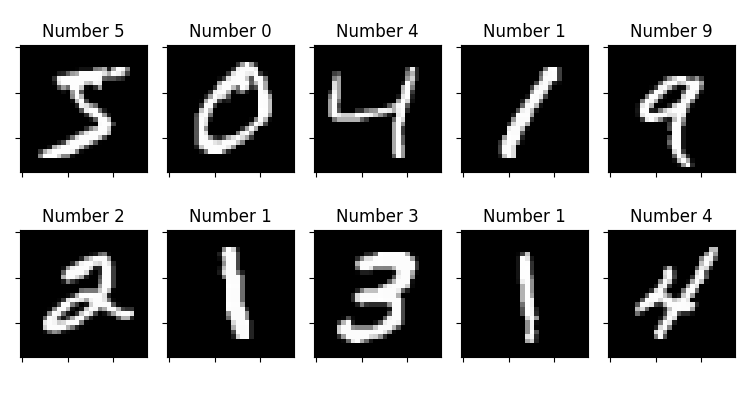
\includegraphics[width=2.5in]{data.png}
\captionsetup{justification=centering}                                                                                         
\caption{The first 10 samples of the train dataset}
\label{fig:data}                                                                                                                               
\end{figure}




The training population presents a distribution with mean $\mu = 6\,000$ and standard deviation $\sigma \simeq 340$ and thus we didn't notice any important unbalance in the data. For this reason we assumed the data followed a distribution $X \sim U(\mu, \sigma)$ and no data augmentation on less populated classes was taken into account. Figure \ref{fig:hist} shows the data distribution for both training and test datasets.

\begin{figure}[ht!]
\centering                                                                        
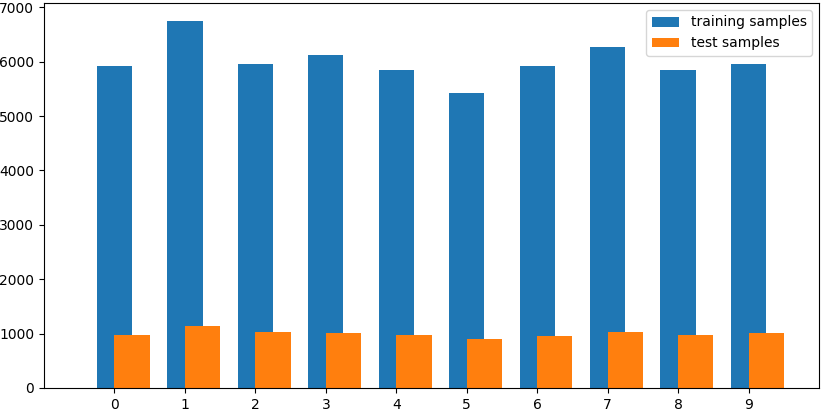
\includegraphics[width=3.5in]{hist.png}
\captionsetup{justification=centering}                                                                                         
\caption{Histogram of the frequency of samples in the dataset}
\label{fig:hist}                                                                                                                               
\end{figure}

\section{Preparing the data}
Before training a FFNN using this images, encoded in $28\times28$ matrices with values from $0$ to $255$, we flattened them in
arrays $1\times784$ and rescaled each value in the continuous interval $[0, 1]$. This encoding will be used in every section of this work: a flat array
better suits the input layer of a FFNN and small values increases the efficiency in the calculations.


\subsection{Data split}
As noted in section \ref{sec:insp}, the dataset is divided into training and test samples. A validation subset is missing and thus
is retrieved from the training set: $15\%$ of the images are randomly used for validation instead of training (along with their labels) for a total of $9\,000$ samples. \par
About labels, we encoded them in one-hot vectors so that the $1$s are set in the index representing the numerical class. \par

\section{Building the network and training}
The aim of this section is to describe a CNN with less than $10\,000$ parameters that is able to classify
with high level of accuracy the numbers from the dataset with or without any regularization technique. Most of the choices were done according to the results
coming from the training and prediction phases.

\subsection{The network}
The CNN presents a typical architecure formed by convolutional layers followed by pooling layers and ending with dense layers. \par
In particular there are 2 convulutional layers covering the whole $28 \times 28$ matrix, formed by 8 $3 \times 3$ filters, for a total dimension of $28 \times 28 \times 8$. These two layers are followed by a max pooling layer that halves the the widht and height of the outcoming activation map. For this problem we tested both \emph{max pooling} and \emph{average pooling}; the first one performed slighty better ($+0.1\%$ in test accuracy): usually \emph{average pooling} smooths out the image and  the sharp features may be identified with more difficulty, while \emph{max pooling} chooses the white pixels of the image (in case of MNIST dataset, the pixels defining the handwritten digit). Although we noticed a slighty improvement using \emph{max pooling}, the images are too small to actually benefit from the methods' differences.
The structure continues with another one convolutional layer aligned with the 2D spatiality of the last pooling layer but doubled in the depth, that is $7 \times 7 \times 16$. The convolutional layer is reduced in spatiality by another \emph{max pooling layer} $7 \times 7 \times 16$ and flattened in a 1D array of $784$. The input flows to an output layer activated by \emph{Softmax} function. Figure \ref{fig:cnn} summarizes the entire architecture and Table \ref{tab:count} highlights the number of parameters in each layer.



\begin{table}[ht!]
\begin{tabular}{|ll|l|}
\hline
\rowcolor[HTML]{3166FF} 
\multicolumn{1}{|l|}{\cellcolor[HTML]{3166FF}{\color[HTML]{FFFFFF} \textbf{Layer}}} & {\color[HTML]{FFFFFF} \textbf{Size}} & {\color[HTML]{FFFFFF} \textbf{Parameters}} \\ \hline
\multicolumn{1}{|l|}{input}                                                         & $28\times28\times1$                          &   $0$                                             \\ \hline
\multicolumn{1}{|l|}{Conv2D-1}                                                      & $28\times28\times8$                           &  $(3\cdot3\cdot1+1)\cdot8 = 80$                                            \\ \hline
\multicolumn{1}{|l|}{Conv2D-2}                                                      & $28\times28\times8$                            &  $(3\cdot3\cdot8 + 1)\cdot8 = 584$                                            \\ \hline
\multicolumn{1}{|l|}{MaxPool-1}                                                     & $14\times14\times8$                            &  $0$                                            \\ \hline
\multicolumn{1}{|l|}{Conv2D-3}                                                      & $14\times14\times16$                            & $(3\cdot3\cdot8 + 1)\cdot16 = 1\,168$                                            \\ \hline
\multicolumn{1}{|l|}{MaxPool-2}                                                      & $7\times7\times16$                            & $0$                                            \\ \hline
\multicolumn{1}{|l|}{Flatten}                                                       & $1\times1\times784$                            & $0$                                            \\ \hline
\multicolumn{1}{|l|}{Dense}                                                         & $1\times1\times10$                            & $(784 + 1)\cdot10 = 7\,850$                                            \\ \hline
\multicolumn{2}{|l|}{\textbf{Total}}                                                                                       &       $9\,682$                                     \\ \hline
\end{tabular}
\caption{Summary of the layers' dimensions and count of the parameters for each layer}
\label{tab:count}
\end{table}



\begin{figure}[ht!]
\centering                                                                        
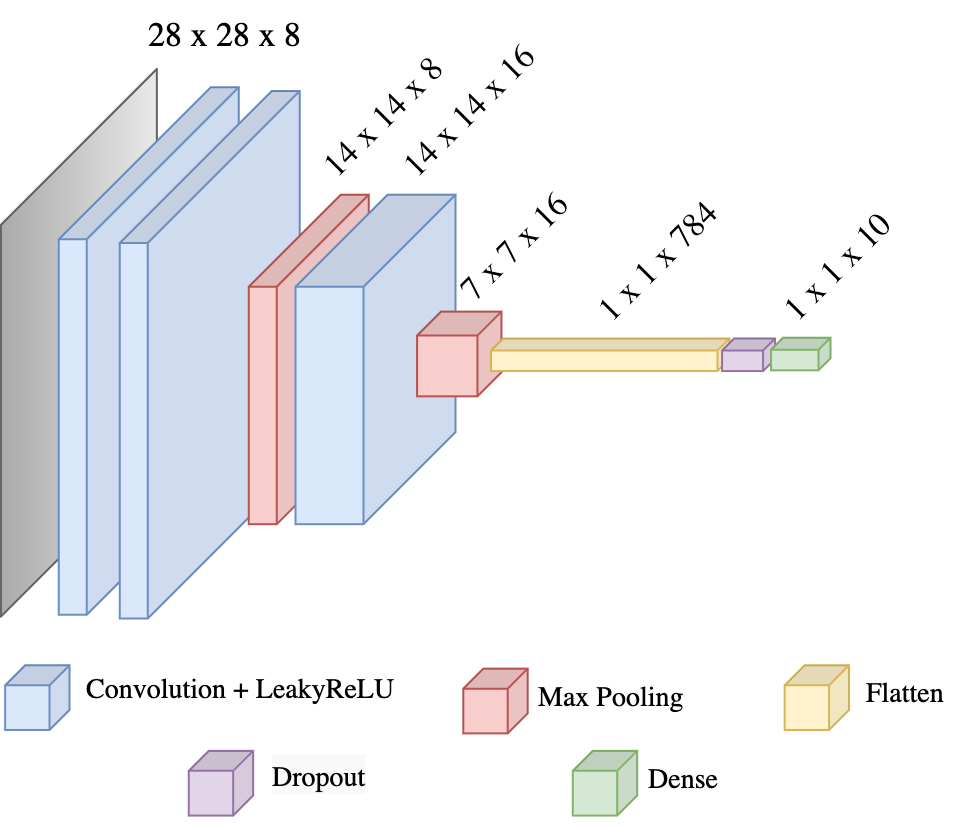
\includegraphics[width=3.5in]{cnn.png}
\captionsetup{justification=centering}                                                                                         
\caption{Architecture of the CNN}
\label{fig:cnn}                                                                                                                               
\end{figure}

About the convulutional layers, Tensorflow allows to specify the padding: no padding and padding with zeroes. The first one would had reduced the spatiality of each layer by $1$, the second one preserves the dimensions by putting evenly $0$s on the margins. Adding $0$s with this particular dataset is not an issue, because most of the images (if not all of them) do not contain information along the margins.
We benchmarked the performances of both methods and we noticed that the zero padding performed had an higher validation accuracy of $+0.8\%$.




\subsection{Training}
The choice of the optimizer was among \emph{SGD} and \emph{Adam}. As expected the first one performed better with small batches (2 to 4), the second one with batches of $256$ samples; 
none have shown signs of getting stuck in local minimum regions but \emph{Adam} performed better overall, with $+1\%$ on test accuracy. \par

The only regularization used is the \emph{dropout} technique applied to the flattened layer with a rate of $40\%$ and \emph{early stopping} during validation. This allowed the model to not overifit too much and generalize better the problem. \par
The behaviour of the model during the training phase is described in the plots of the loss and categorical accuracy in 
Figure \ref{fig:loss} and Figure \ref{fig:acc}. 
It easy to find out that the model converges after $14$ epochs and the \emph{early stopping} mechanism stopped the learning process after $24$ epochs (out of maximum of $50$). The \emph{early stopping} had a patience factor of 10 with a minimum $\delta$ of $0.5\%$ in validation accuracy.
We didn't resumed the model's weight at the $14^{th}$ epoch because its training accuracy ($98.01\%$) wasn't too distant from the final one ($98.44\%$) and gave the possibility to the validation accuracy to raise from $97.82\%$ to $98.98\%$.
\begin{figure}[ht!]
\centering                                                                        
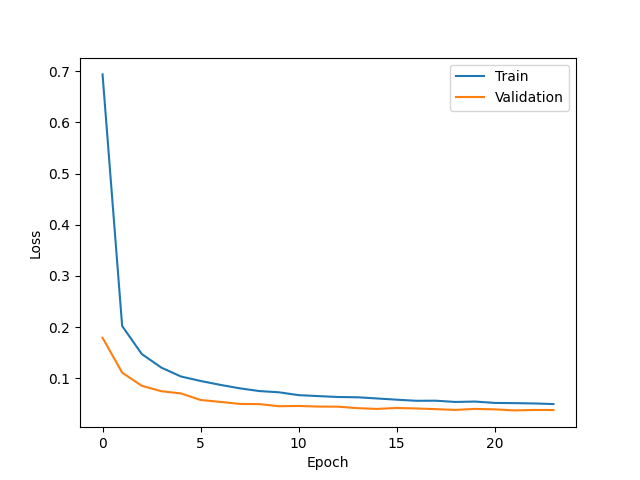
\includegraphics[width=3.5in]{loss.png}
\captionsetup{justification=centering}                                                                                         
\caption{Loss}
\label{fig:loss}                                                                                                                               
\end{figure}


\begin{figure}[ht!]
\centering                                                                        
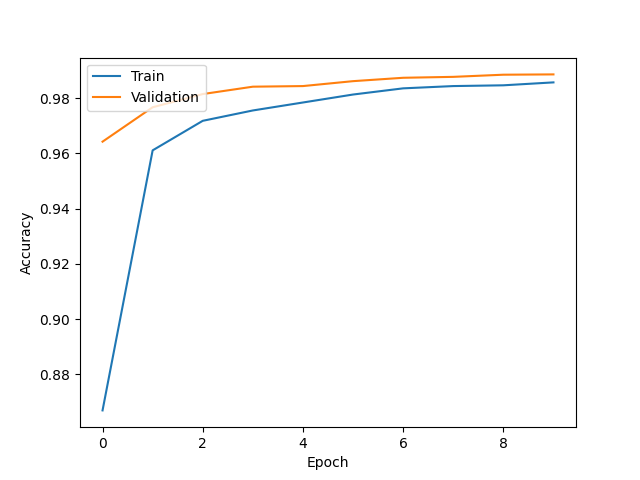
\includegraphics[width=3.5in]{acc.png}
\captionsetup{justification=centering}                                                                                         
\caption{Categorical accuracy}
\label{fig:acc}                                                                                                                               
\end{figure}

The validation loss was always lower than the training loss. This is effect is caused by the \emph{dropout} because it penalizes model variance by randomly removing neurons from the flatten layer only during the training; the models underfitted and since \emph{dropout} is disabled during the validation we had lower validation loss. The same for the accuracy, being higher during validation.\par
The best validation accuracy reached was $98.98\%$ using \emph{Adam} with learning rate of $10^{-3}$ and batch size of $256$.


\subsection{Evaluation}
We tested the quality of the model's predictions using the provided test dataset, applying very same transormations on the images used for the training.
The categorical accuracy 
over the test set reached $98.65\%$ and can be analyzed with the help of the confusion matrix (Figure \ref{fig:cm}). 

\begin{figure}[ht!]
\centering                                                                        
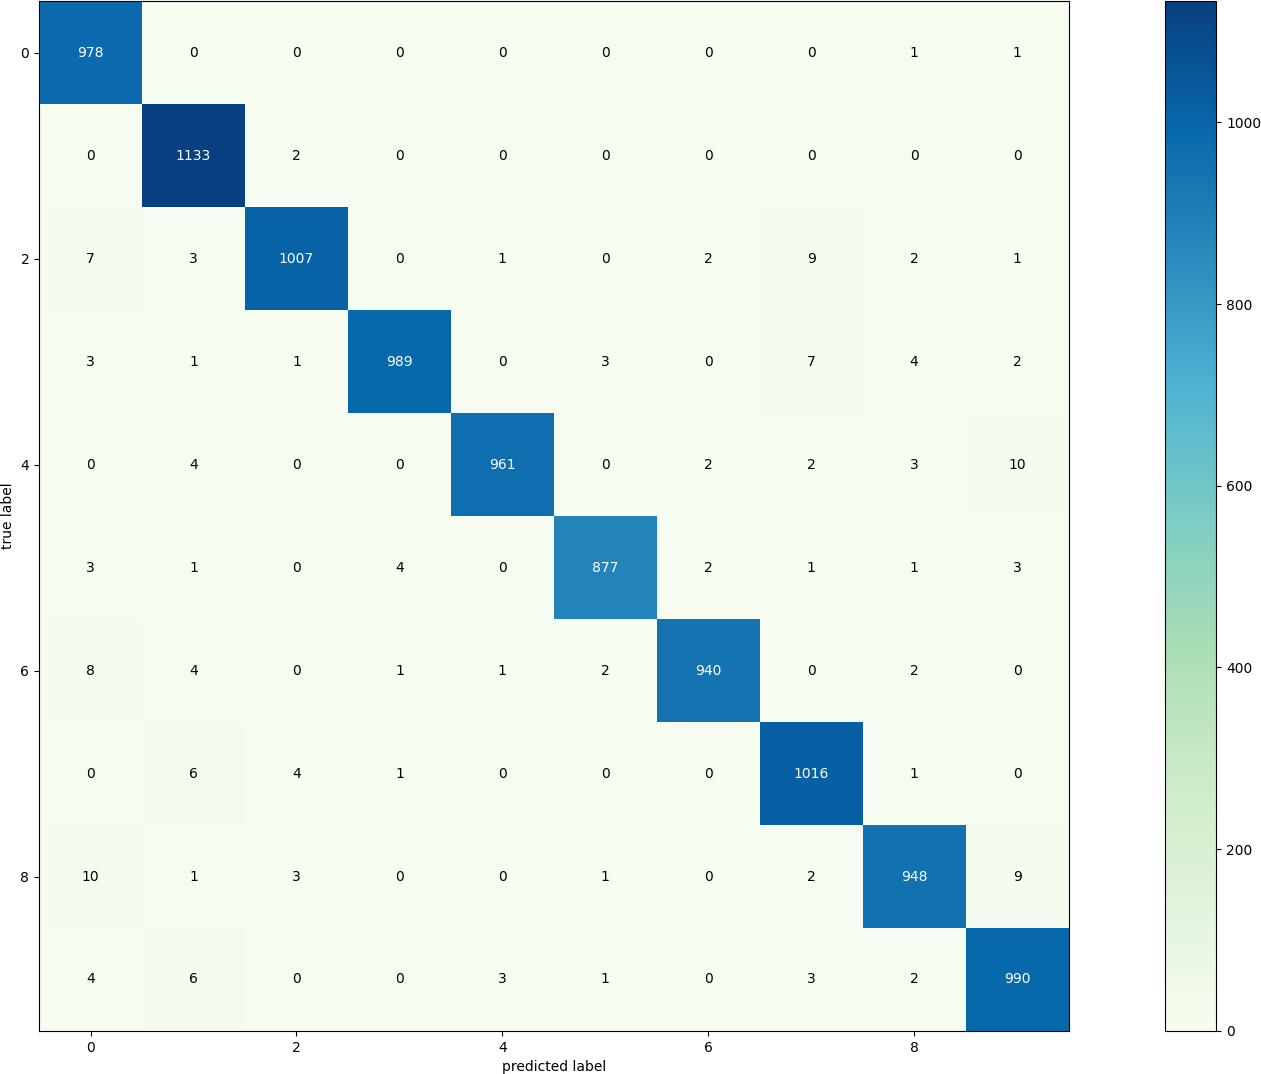
\includegraphics[width=3.5in]{cm2.png}
\captionsetup{justification=centering}                                                                                         
\caption{Confusion matrix over the test data}
\label{fig:cm}                                                                                                                               
\end{figure}

We noticed that the model confused the $2.34\%$ of the $4$s with a $9$: this can be explained by the fact that the two digits have similar forms, in particular when
the $4$ is written quicky and in its \emph{"closed form"}. Another source of confusion is the $8$ beign confused again with a $9$ ($1\%$ of the cases). Apart from these cases, that have a realitively low impact, the model gave really good results.


\end{document}









